\section{Estado del arte}

En este apartado daremos un definición general sobre qué es la generación procedimental de contenidos, dónde y para qué se usa; haremos un recorrido histórico desde los precursores de la \acrshort{pcg} hasta la actualidad; y finalmente entraremos a tratar con más detalle la \acrshort{pcg} en los videojuegos, estableciendo una clasificación del contenido generado y de los métodos más utilizados en \acrshort{pcg}.

\subsection{Generación procedimental de contenidos (PCG)}

\subsubsection{¿Qué es la PCG?}

Antes de comenzar, debemos describir qué es la \acrshort{pcg}. En nuestro caso partiremos de la definición dada en 2015 por Gillian Smith, en el que define la \acrshort{pcg} como: \\

\say{\textit{El uso de un algoritmo formal para generar contenido [...] que normalmente sería producido por un humano}}\cite{smith2015}.\\

Debido al uso de algoritmos, es un error frecuente su asociación con los videojuegos, la animación y los ordenadores en general. Aunque es cierto que sus usos más comunes son la creación de modelados y texturas o la automatización de la generación de grandes cantidades de contenido en un juego, la \acrshort{pcg} se ha usado y se usa en otros campos como la música que veremos a continuación.\\

Si lo orientamos al ámbito de los juegos, es interesante como Smith \cite{smith2015} no establece la \acrshort{pcg} como un problema que se podría enmarcar únicamente en el ámbito de la inteligencia artificial (\acrshort{ai} por su sigla en inglés, \acrlong{ai}), cuyo objetivo sería el de reemplazar o imitar el contenido generado por un diseñador humano, sino que lo establece como un problema más amplio que se superpone con el diseño de juegos, pudiendo ser aplicada la \acrshort{pcg} tanto por ordenadores como por humanos.\\

\begin{figure}[H]
    \begin{center}
        \begin{subfigure}[b]{0.24\textwidth}
            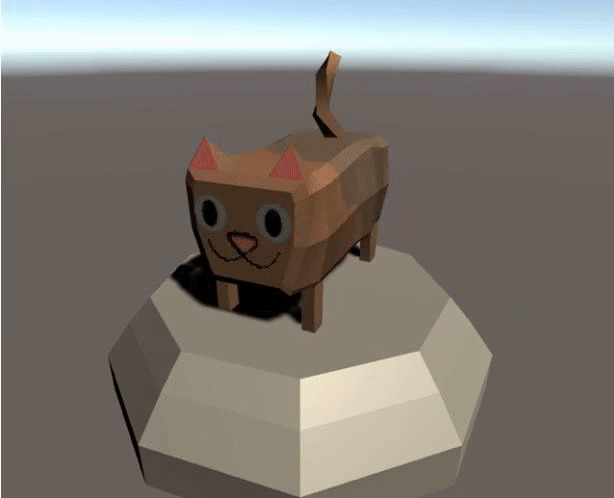
\includegraphics[width=\textwidth]{img/cat1.jpg}
        \end{subfigure}
        \hfill
        \begin{subfigure}[b]{0.24\textwidth}
            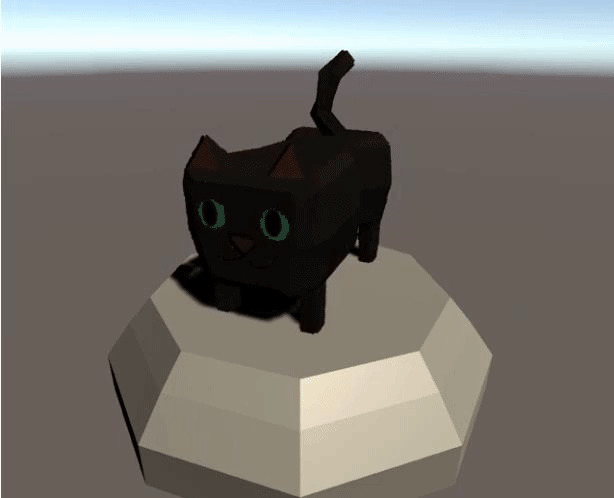
\includegraphics[width=\textwidth]{img/cat2.jpg}
        \end{subfigure}
        \hfill
        \begin{subfigure}[b]{0.24\textwidth}
            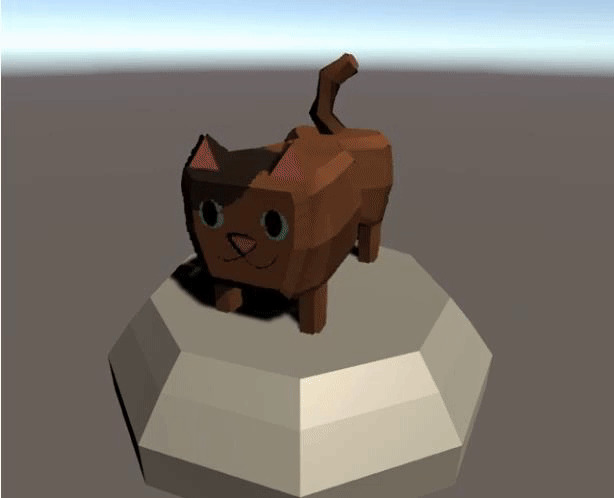
\includegraphics[width=\textwidth]{img/cat3.jpg}
        \end{subfigure}
        \hfill
        \begin{subfigure}[b]{0.24\textwidth}
            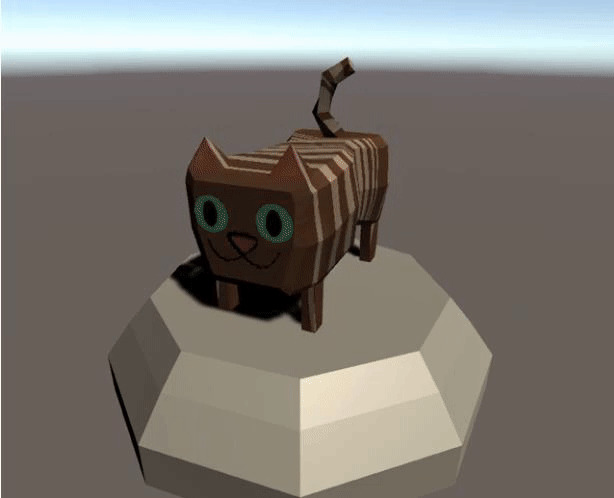
\includegraphics[width=\textwidth]{img/cat4.jpg}
        \end{subfigure}
        \caption{Modelo 3D de un gato en el que se elige semi-aleatoriamente los parámetros del pelaje. Imagen obtenida de \cite{collins2017}}
    \end{center}
\end{figure}

\subsubsection{¿Dónde y para qué se utiliza la PCG?}

La \acrshort{pcg} no solo tiene cabida en el ámbito de los videojuegos. Desde hace décadas se ha utilizado en juegos de mesa de rol (\acrshort{rol} por su sigla en inglés, \acrlong{rol}), en el cine o incluso para componer música.\\

Probablemente el ejemplo más conocido de \acrshort{rol} sea Dragones y Mazmorras (\acrshort{dyd} por su sigla en inglés, \acrlong{dyd}). En 1976, TSR Hobbies lanzó \say{\textit{Dungeon geomorphs}}, un conjunto de baldosas que permitía crear de manera procedimental gran variedad de mazmorras, similar al de la figura \ref{fig:dyd}. Las baldosas estaban diseñadas de tal modo que permitía conectar unas con otras con facilidad, cumpliendo con el objetivo principal de la \acrshort{pcg}, y es el de generar contenido jugable. Es interesante como ya en aquel entonces las instrucciones de uso de \say{\textit{Dungeon geomorphs}} invitaba al usuario a anotar el resultado obtenido con las baldosas y a realizar las modificaciones que creyese convenientes, introduciendo un elemento de vital importancia, y es la posibilidad del usuario de intervenir en el proceso y modificar el contenido generado procedimentalmente. Otro gran ejemplo de aleatoriedad guiada es la generación de encuentros y de mazmorras que también presenta \acrshort{dyd}, en su guía \say{\textit{Advanced Dungeons \& Dragons}}, utilizando lanzamientos de dados y tablas de contenido \cite{smith2015}.\\

\begin{figure}[H]
    \begin{center}
        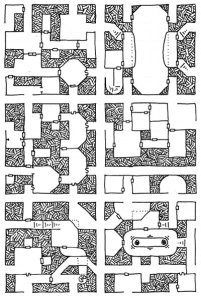
\includegraphics[scale=3, angle =90 ]{img/dungeon_geo.jpg}
        \caption{Conjunto de baldosas similar a los lanzados por TSR Hobbies en 1976. Imagen obtenida de \cite{dungeonTiles}.}
        \label{fig:dyd}
    \end{center}
\end{figure}

Un uso menos conocido de la \acrshort{pcg} es el de la generación de música y sonido. Un ejemplo de este uso es el artista Brian Eno, quién popularizó el término \say{\textit{generative music}} \cite{eno1996}. Un ejemplo más cercano es el que nos da Chister Kaitila en su breve tutorial \say{\textit{Procedural Music Generation}}, creado para la PROCJAM 2017, en el que define varias reglas para generar música procedimentalmente dónde compara la música con mazmorras y las frases musicales con las habitaciones de la mazmorra \cite{kaitila2017}.

\newpage
Fuera del mundo de los juegos, un campo en el que el uso de técnicas de \acrshort{pcg} es más frecuente de lo que podría parecer inicialmente es el cine. MASSIVE \cite{massive} es un software de generación procedimental que se creó originalmente para la trilogía del Señor de los Anillos que permite añadir miles de individuos a una escena, reduciendo el trabajo de meses a días \cite{collins2017}.\\

Este software se ha usado en multitud de películas y series como \textit{Avatar (2009)}, en la que se añadió árboles y plantas a las vastas selvas de Pandora; \textit{Guerra Mundial Z (2013)}, en la que se simularon las hordas de no-muertos o se añadió extras a las escenas tomadas en el portaaviones; \textit{La Gran Muralla (2016)}, en la que se simularon escenas con más de 300 mil criaturas; el capítulo titulado \say{\textit{La Batalla de los Bastardos}}\textit{ (2016)} de la serie \textit{Juego de Tronos}, en el que se simuló los choques de ambos ejércitos, incluyendo infantería y caballería, serie de la que podemos ver una escena antes y después de aplicar este software en la figura \ref{fig:massive}.\\

El uso de este software ha permitido un ahorro de tiempo colosal en el desarrollo de estas y muchas más obras cinematográficas, ya sea generando y simulando el comportamiento de grupos multitudinarios de entidades o dando vida a escenas en las que si no hubiera sido por este tipo de técnicas, hubiese requerido de una mayor inversión de dinero y esfuerzo.\\

\begin{figure}[H]
    \begin{center}
        \begin{subfigure}[b]{0.49\textwidth}
            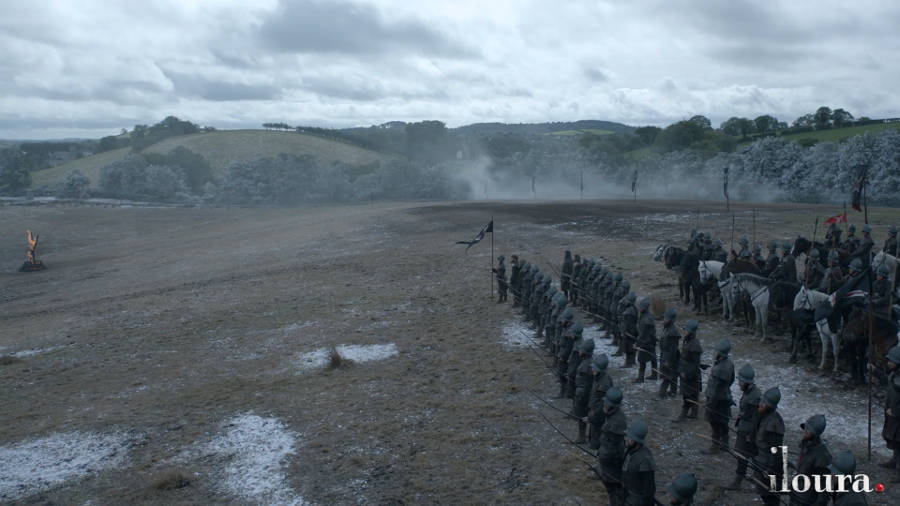
\includegraphics[width=\textwidth]{img/got_before.jpg}
            \caption{Escena antes de usar MASSIVE.}
        \end{subfigure}
        \hfill
        \begin{subfigure}[b]{0.49\textwidth}
            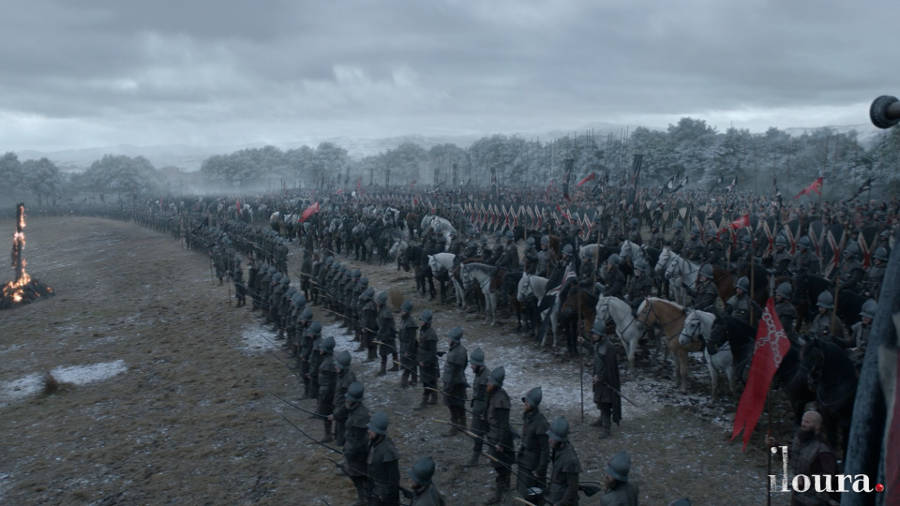
\includegraphics[width=\textwidth]{img/got_after.jpg}
            \caption{Escena tras usar MASSIVE.}
        \end{subfigure}
        \caption{Uso del software MASSIVE en la serie \textit{Juego de Tronos}. Imagen obtenida de \cite{massive}.}
        \label{fig:massive}
    \end{center}
\end{figure}

Volviendo al ámbito de los videojuegos, en sus trabajos \cite{smith2014}, \cite{smith2015} Smith habla de la utilización de métodos de \acrshort{pcg} con el fin de producir gran variedad de elementos, pasando por niveles, mapeado o texturas hasta llegar al contenido de la propia historia del videojuego. Además de la creación de contenido prácticamente ilimitado con el fin de crear una sensación de rejugabilidad en los jugadores, Smith nombra otros motivos de peso para usar \acrshort{pcg} en el desarrollo de un videojuego, ya que por ejemplo puede proporcionar un contenido que se adapte mejor al jugador. No es de extrañar que Smith centre su trabajo hacia la creación de mejores experiencias para el usuario ya que como ya hemos dicho, entiende el problema como algo más allá del campo de la \acrshort{ai}.

% ---------------------------------------------------------------------------- %

\subsection{PCG en los videojuegos}

\subsubsection{Clasificación de contenido generado procedimentalmente}

En sus trabajos sobre generación procedimental aplicada a los videojuegos Hendrikx \textit{et al.} \cite{hendrikx2013} y más tarde Barriga \cite{barriga2019} establecen una clasificación para el contenido generado procedimentalmente que se divide en las siguientes seis categorías:

\begin{enumerate}[label=(\alph*)]
    \item \textbf{Game Bits:} son las unidades más básicas de contenido de un juego. Habitualmente se trata de elementos que no interaccionan directamente con el usuario. A su vez, Hendrikx \textit{et al.} subdividen esta categoría en otros seis tipos de \textit{Game Bits}:
    
    \begin{itemize}
        \item \textit{Texturas:} se tratan de las imágenes que se utilizan para añadir detalle a las geometrías y modelos, representando habitualmente los materiales de los que están compuestos los distintos objetos del juego. En la actualidad, debido a la cantidad de esfuerzo necesario para crear texturas realistas, muchos juegos han optado por técnicas de \acrshort{pcg} para crear las texturas más generales mientras que utilizan a los artistas para generar las texturas más complejas. Podemos ver un ejemplo de una textura generada procedimentalmente en la figura \ref{fig:voronoi}.
        
        \begin{figure}[H]
            \begin{center}
                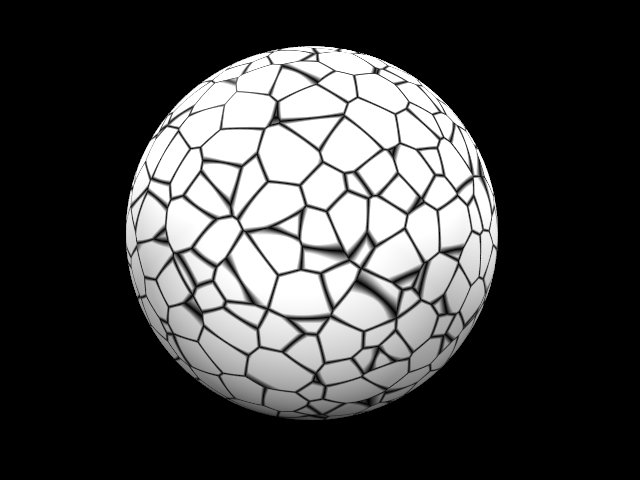
\includegraphics[scale=0.3]{img/Blender3D_VoronoiCrackle.jpg}
                \caption{Textura \textit{``fracturada''} generada procedimentalmente utilizando Teselación de Voronoi. Imagen obtenida de \cite{voronoi2007}.}
                \label{fig:voronoi}
            \end{center}
        \end{figure}
        
        \item \textit{Sonido:} tiene una función primordial en la experiencia de juego, ya que la música ayuda a establecer la atmósfera y ritmo del juego, mientras que los efectos de sonido se utilizan para dar información al usuario en función de sus acciones o de los cambios de usuario. Actualmente, los juegos dependen principalmente de clips de sonido pregrabados que se reproducen en función de los eventos del juego \cite{manocha2009}. Por otra parte, la generación procedimental aplicada a este campo no tiene una gran acogida, ya que la producción de música mediante algoritmos todavía genera animadversión entre el público y los propios compositores debido a la falsa creencia de que el ordenador es el responsable de dicha obra y no el compositor \cite{edwards2011}.
        \item \textit{Vegetación:} el uso de vegetación, además de su componente claramente visual, puede interactuar con el jugador ya sea sirviendo como lugar de cobertura o dando información al mismo, creando entornos realistas e inmersivos. Podemos ver un ejemplo de varios árboles generados procedimentalmente en la figura \ref{fig:arboles}.
        
        \begin{figure}[H]
            \begin{center}
                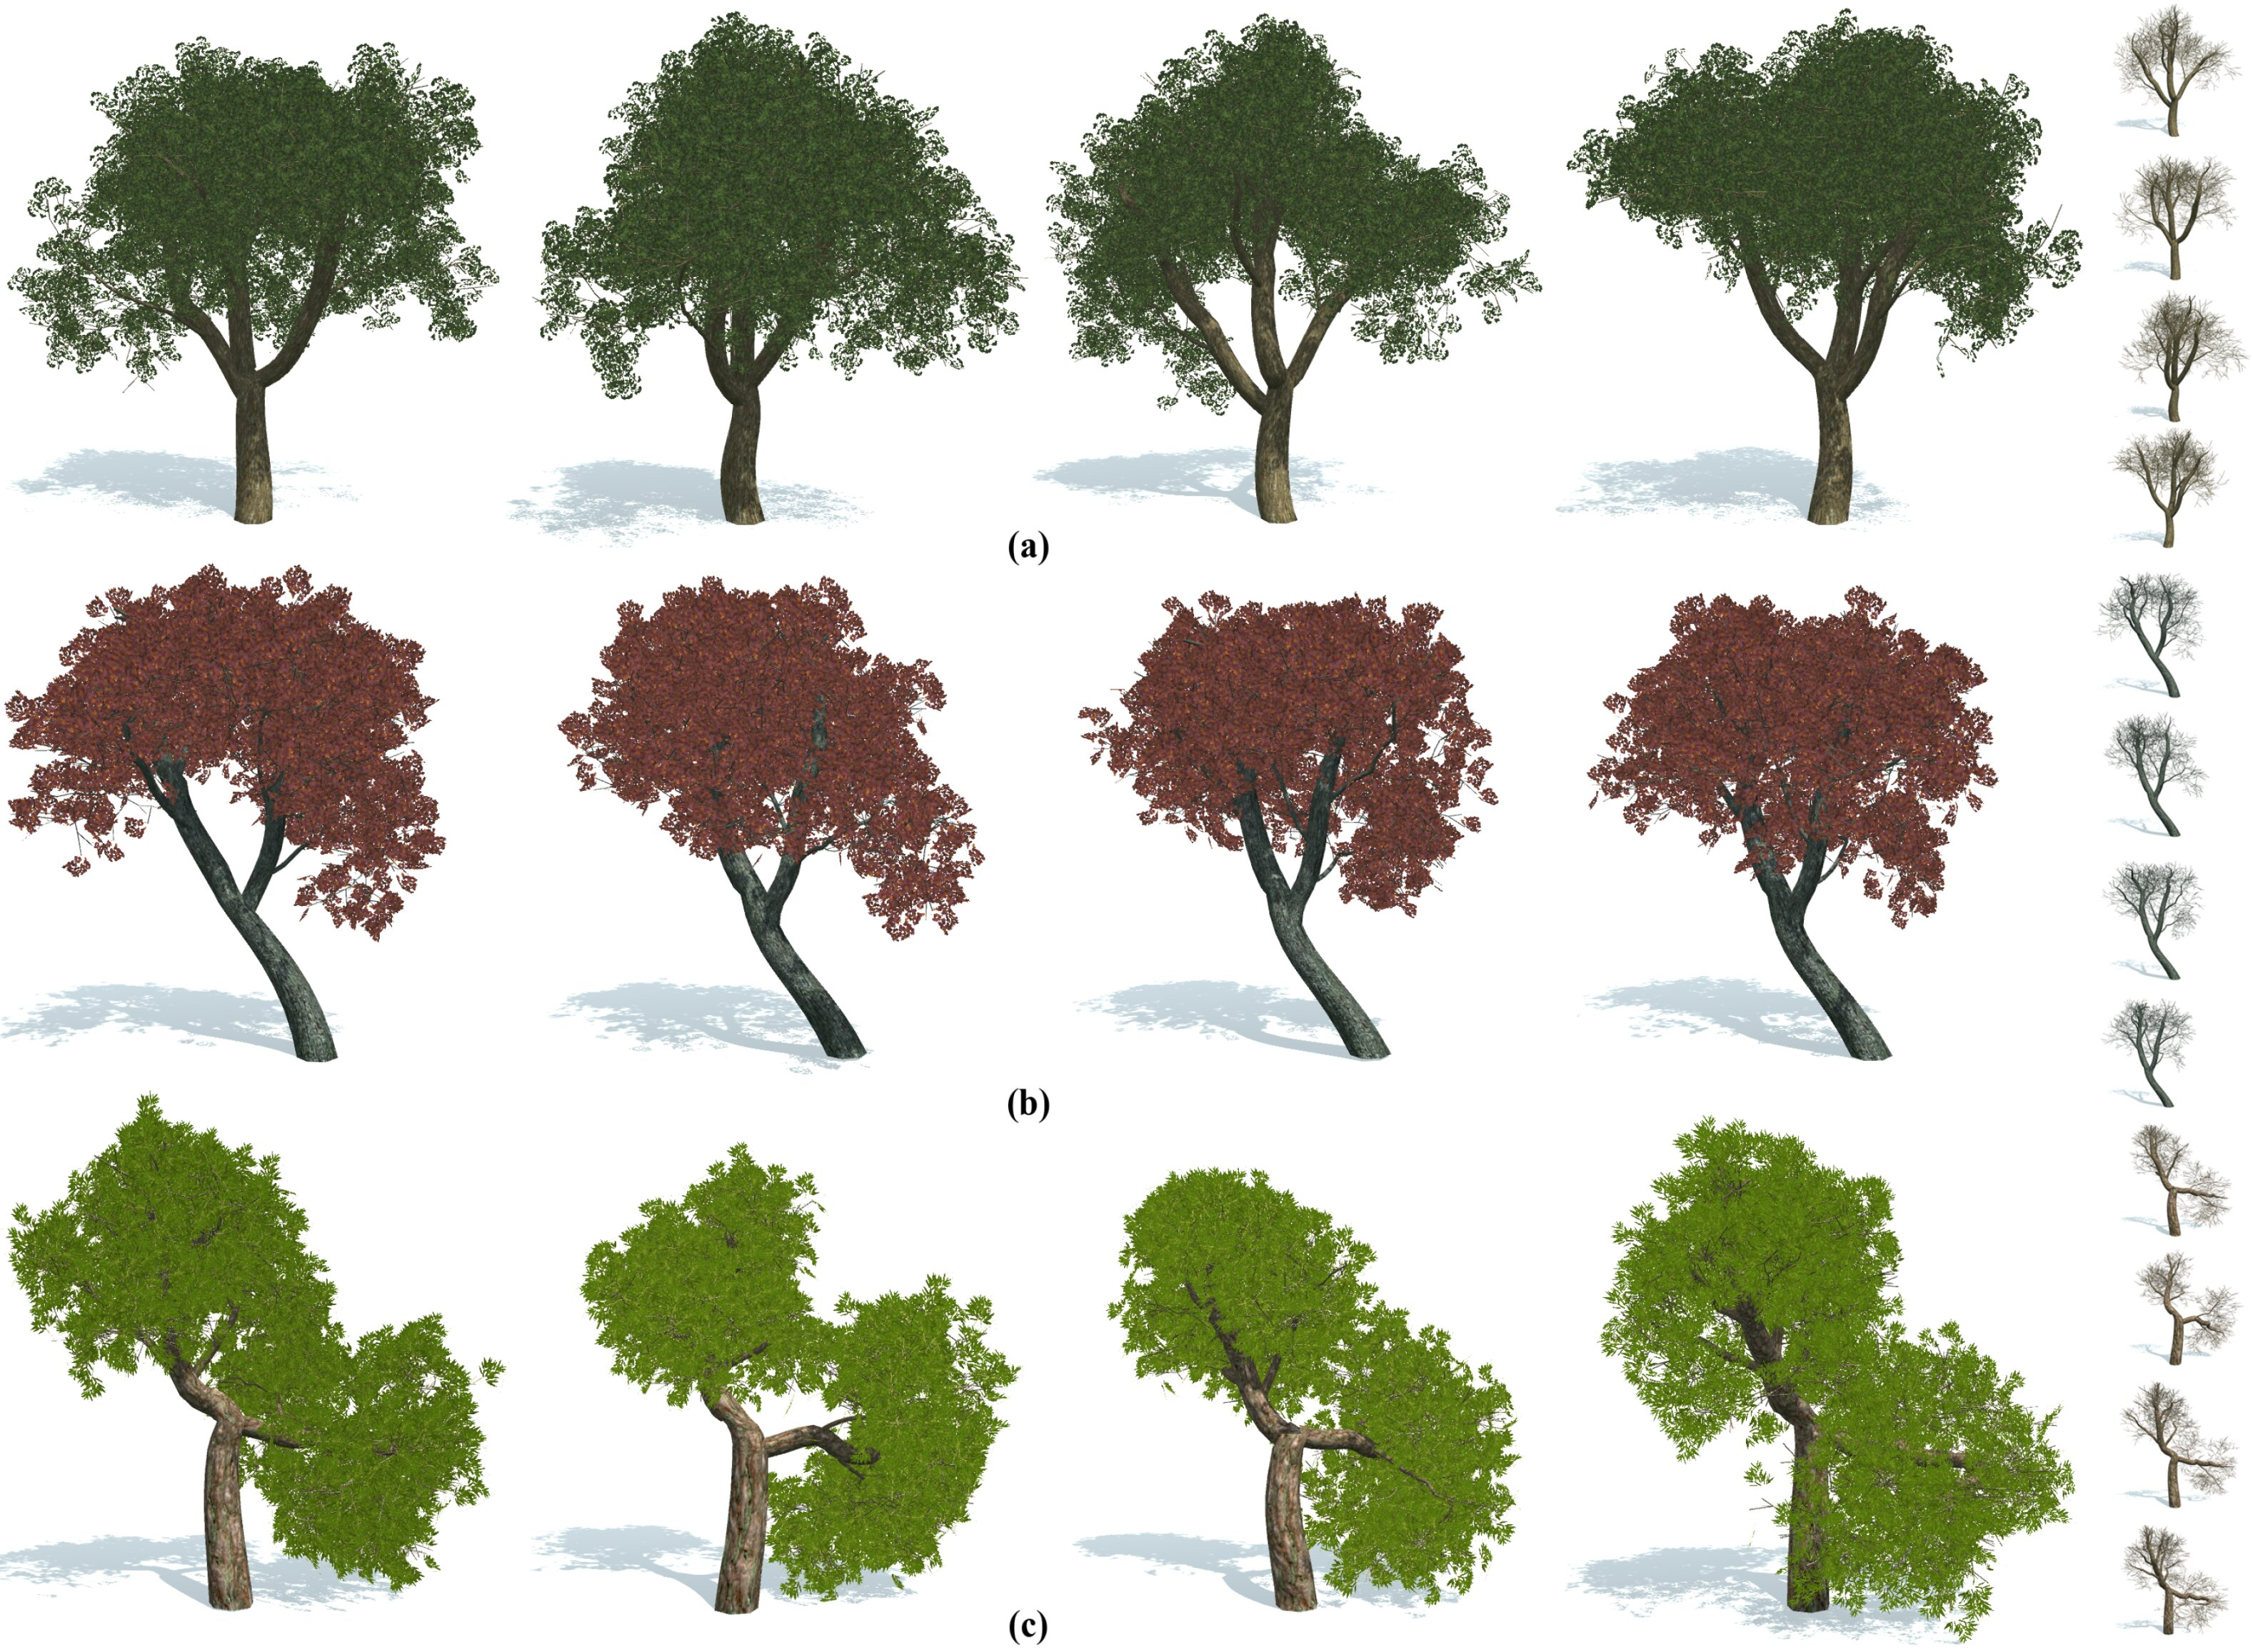
\includegraphics[scale=0.08]{img/tree-models.jpg}
                \caption{Diversos modelos de árboles generados utilizando el algoritmo procedimental propuesto por Jinmo Kim. Imagen obtenida de \cite{kim2016}.}
                \label{fig:arboles}
            \end{center}
        \end{figure}        
        
        \item \textit{Edificaciones:} al igual o más que la vegetación, los edificios ayudan a dar información al jugador del mundo que les rodea, siendo necesaria variedad en la generación de los mismos para mantener la inmersión del jugador.
        \item \textit{Comportamiento:} refiriéndose al modo en el que los objetos interaccionan entre sí y con el entorno que les rodea. Los comportamientos generados procedimentalmente permiten crear la ilusión de un entorno complejo.
        \item \textit{Elementos:} al igual que el resto de \textit{Game Bits}, los elementos como son el agua, el fuego, el viento o la tierra se utilizan para crear un entorno más realista. Con los avances computacionales y de modelado, estos han pasado de tener un papel meramente decorativo a una representación realista de los mismos y como interactúan con el mundo.
    \end{itemize}
    
    \item \textbf{Game Space:} es el entorno en el que el juego se desarrolla, en el que Hendrikx \textit{et al.} \cite{hendrikx2013} solo consideran como \textit{Game Space} a las zonas uni-, bi-, o tri-dimensionales de nuestro juego en las que están situados elementos con una posición y dirección relativa.
    
    \begin{itemize}
        \item \textit{Mapeado:} mientras Hendrikx \textit{et al.} \cite{hendrikx2013} hablan tanto de mapeado interior como exterior, Barriga \cite{barriga2019} lo simplifica unificando ambas categorías en una sola. Un ejemplo sería una mazmorra de un dungeon-crawler\footnote{Son juegos que consisten en recorrer una mazmorra, habitualmente recogiendo botín y eliminado enemigos.} como el juego \textit{Darkest Dungeon} que genera procedimentalmente la distribución y contenido de las habitaciones de la mazmorra que debe recorrer el jugador, como se puede observar en la figura \ref{fig:darkdungeon}.
        
        \begin{figure}[H]
            \begin{center}
                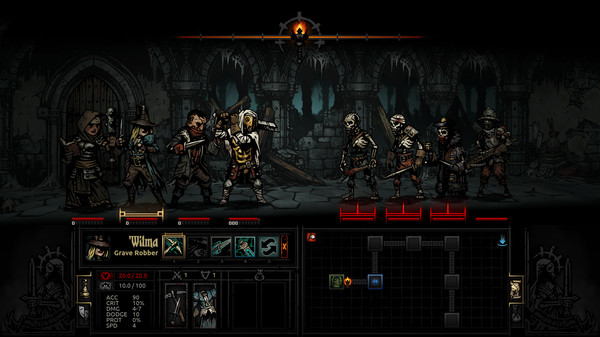
\includegraphics[scale=0.65]{img/darkest.jpg}
                \caption{En el juego \textit{Darkest Dungeon}, la distribución y contenido de la mazmorra se genera cada vez que entramos en ella. Imagen obtenida de \cite{redhook}.}
                \label{fig:darkdungeon}
            \end{center}
        \end{figure}   
        
        \item \textit{Terreno:} incluyendo elementos como ríos, lagos, mares, montañas, barrancos, grutas, etc. al igual que otros como podrían ser las zonas de teletransporte. Un ejemplo es la generación del terreno en el juego \textit{No Man's Sky}, juego en el que cada planeta que visitemos contará con distintos elementos geográficos.
    \end{itemize}
    
    \item \textbf{Game Systems:} se trata de la simulación de entornos más complejos que los representados en la categoría anterior. Un buen sistema consigue crear juegos más realistas y creíbles, por lo que son más atractivos para el consumidor. En este caso, dividimos esta categoría en cuatro tipos:
    
    \begin{itemize}
        \item \textit{Entornos urbanos:} el principal enfoque para la generación procedimental de grandes grupos de edificios primero pasa por generar las ya mencionadas redes de carreteras para a continuación generar los edificios.
        \item \textit{Comportamiento de entidades:} por último, es necesario crear entornos en los que la interacción de las distintas entidades entre sí y el jugador sean realistas y parezcan vivos. El uso de personajes no jugables (\acrshort{npc} por su sigla en inglés, \acrlong{npc}) es una de las herramientas más potentes de cara a crear estos entornos inmersivos, ya que no solo es importante una interacción realista del jugador con el resto de elementos del juego. Un claro ejemplo de situación en la que los algoritmos procedimentales pueden lograr un resultado realista es en los patrones de movimiento de grupos de individuos, como ocurre en el videojuego \textit{ S.T.A.L.K.E.R.: The Shadow of Chernobyl} \cite{amato2017}.
        \item \textit{Ecosistemas:} definen la manera en la que interaccionan flora y fauna en base a una serie de algoritmos y reglas. Esto nos permite crear sistemas en los que exista una evolución de los individuos, una definición de sus hábitats o cadenas tróficas realistas. Podemos ver un ejemplo de un ecosistema compuesto por flora y fauna generados procedimentalmente en la figura \ref{fig:noman}.
        
        \begin{figure}[H]
            \begin{center}
                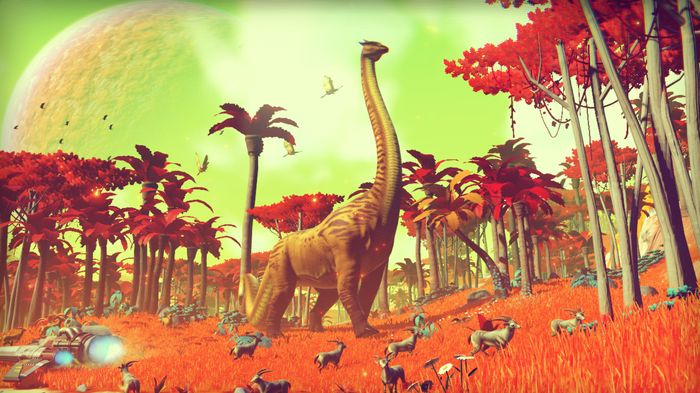
\includegraphics[scale=0.4]{img/no-mans-sky.jpg}
                \caption{En el juego \textit{No Man's Sky}, los ecosistemas de cada planeta son generados procedimentalmente. Imagen obtenida de \cite{grendel-games}.}
                \label{fig:noman}
            \end{center}
        \end{figure}    
        
        \item \textit{Redes de carreteras:} son la estructura básica de comunicación entre los distintos puntos de interés de nuestro mapeado. La dificultad de generar redes de carreteras de manera procedimental es la búsqueda de equilibrio entre la aleatoriedad y el cumplir con una estructura lógica en la disposición de nuestros elementos. Este será uno de los tipos de contenido que generaremos en este proyecto.
    \end{itemize}
    
    \item \textbf{Game Scenarios:} en este apartado encontraríamos los tres niveles anteriores organizados de tal modo que forman planes coherentes o secuencias de eventos. Podemos distinguir claramente cuatro categorías en las que dividir los \textit{Game Scenarios}:
    
    \begin{itemize}
        \item \textit{Guiones gráficos:} principalmente utilizan el formato de viñeta y sirven de ayuda para guiar a los desarrolladores o al propio jugador. En función del modo en el que se usen podremos incluirlo en esta categoría o en la categoría \textit{Derived Content}.
        \item \textit{Historia:} normalmente es la pieza fundamental para crear historias que mantengan al jugador motivado, establecer un sentido lógico a los eventos del juego y proporcionar la meta principal que debe alcanzar nuestro jugador.
        \item \textit{Puzzles:} son problemas a los que el jugador debe encontrar una solución basada en sus conocimientos previos o en la información obtenida al explorar el entorno. Dependiendo del tamaño del problema que se plantee y de la experiencia previa del jugador variará la dificultad asociada al mismo. Un gran ejemplo, visible en la figura \ref{fig:minimotor} es el juego \textit{Mini Metro}, que genera procedimentalmente los niveles, generando puzzles distintos cada vez que se juega y teniendo como objetivo alcanzar la máxima puntuación posible.
        
        \begin{figure}[H]
            \begin{center}
                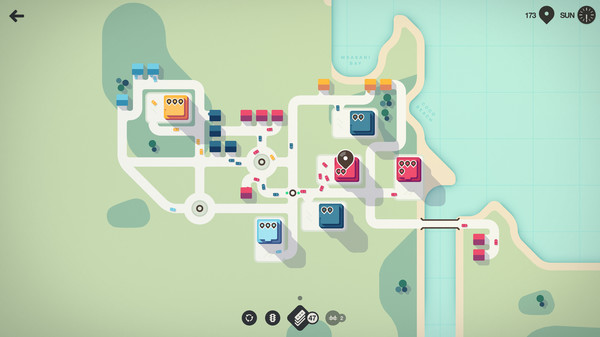
\includegraphics[scale=2]{img/minimotor.jpg}
                \caption{En el juego \textit{Mini Motorways}, la distribución de casas y centros comerciales se genera procedimentalmente. Imagen obtenida de \cite{dinosaurPolo}.}
                \label{fig:minimotor}
            \end{center}
        \end{figure}    
        
        \item \textit{Niveles:} su definición más usada es la de separador entre las distintas secuencias del juego. Son aquellas zonas jugables dónde el jugador debe ir del punto A al punto B, cumpliendo una serie de objetivos por el camino. Podemos ver un ejemplo de nivel generado procedimentalmente del juego \textit{Bad North} en la figura \ref{fig:badnor}, aplicando técnicas \acrshort{pcg} a la generación de niveles en \acrshort{3d}. Este será uno de los tipos de contenido que generaremos en este proyecto.
    \end{itemize}
    
        \begin{figure}[H]
            \begin{center}
                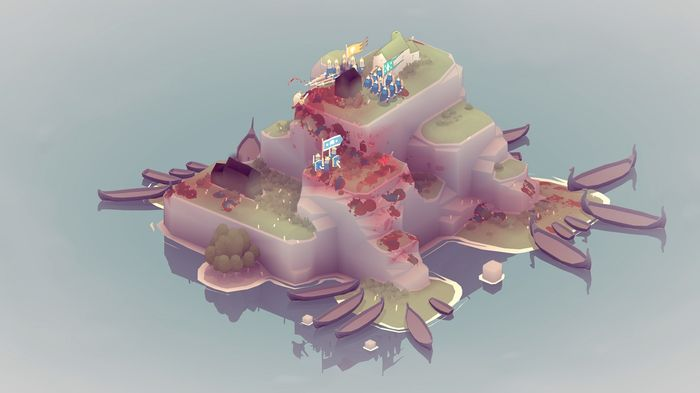
\includegraphics[scale=0.4]{img/bad_north.jpg}
                \caption{En el juego \textit{Bad North}, cada nivel se genera mediante un método conocido como colapso de la función de onda. Imagen obtenida de \cite{grendel-games}.}
                \label{fig:badnor}
            \end{center}
        \end{figure}     
    
    \item \textbf{Game Design:} son las mecánicas y reglas del juego, estableciendo lo que se puede hacer en el juego y lo que no. Tal y como definen en su trabajo Hendrikx \textit{et al.} esta categoría incluye y referencia a todo el contenido ya descrito, incluso de manera recursiva a otro contenido perteneciente al \textit{Game Design}. Todo este contenido puede ser generado automáticamente o de tal modo que proporcione herramientas a los diseñadores.
    \item \textbf{Derived Content:} definiendolo brevemente se trata del contenido que se crea paralelamente al mundo del juego, creando un gran sentido de inmersión en el jugador ya que refleja las acciones y experiencia del usuario dentro y fuera del propio juego.
\end{enumerate}

De esta clasificación en forma de pirámide debemos destacar que los elementos complejos de los niveles superiores suelen estar compuestos de los elementos más simples de los elementos inferiores. Además, debemos dejar claro que aunque algunos de estos elementos son necesarios, otros simplemente son opcionales y no tienen por qué formar parte del desarrollo de un videojuego. Debemos recalcar de nuevo la importancia de un contenido de calidad a la hora de crear entornos inmersivos para el jugador.\\

\begin{figure}[H]
    \begin{center}
        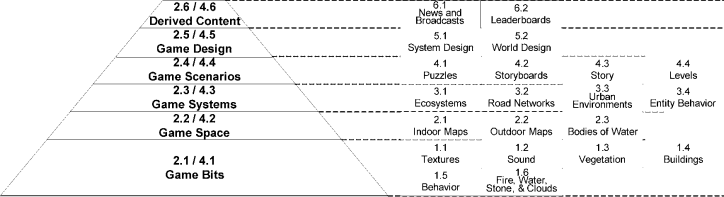
\includegraphics[scale=0.8]{img/hendrikx2013.png}
        \caption{Clasificación piramidal del contenido generado procedimentalmente. Imagen obtenida de \cite{hendrikx2013}.}
    \end{center}
\end{figure}

\subsubsection{Propiedades deseables del PCG}

Dependiendo del problema al que nos enfrentemos y el objetivo que busquemos alcanzar, los métodos de \acrshort{pcg} contaran con distintas características y propiedades. Habitualmente estas características no serán alcanzables a la vez, como ejemplo, podemos implementar un algoritmo muy rápido pero que no asegure la máxima calidad del contenido generado. En el libro de Shaker \textit{et al.} \cite{shaker2016} hablan de las siguientes características deseables de los algoritmos de \acrshort{pcg}:

\begin{itemize}
    \item \textbf{Velocidad:} refiriéndose al tiempo que tarda el algoritmo en generar contenido. Dependiendo del problema, podríamos necesitar una solución en milésimas de segundo a poder permitirnos esperar durante horas.
    \item \textbf{Fiabilidad:} refiriéndose a la precisión con la que garantiza el algoritmo que el contenido generado es de calidad. Mientras que en ocasiones necesitaremos que el contenido no contenga errores, por ejemplo, en la generación de un laberinto, en otras ocasiones, no nos importará sacrificar parte de la calidad del contenido a cambio de velocidad, por ejemplo, en la generación de vegetación.
    \item \textbf{Controlabilidad:} refiriéndose a la posibilidad de una persona u otro algoritmo de modificar o condicionar los resultados obtenidos por el método de \acrshort{pcg}.
    \item \textbf{Diversidad:} refiriéndose a la capacidad de generar contenido variado y que no se base en simples variaciones. Normalmente no es trivial conseguir diversidad sin afectar a la calidad del contenido.
    \item \textbf{Credibilidad:} refiriéndose a la capacidad de imitar al contenido generado por humanos y que no parezca que el contenido generado ha sido creado utilizando algoritmos de \acrshort{pcg}.
\end{itemize}

\subsubsection{Métodos de generación de contenido}

En cuanto a la clasificación de los distintos algoritmos no existe un convenio de categorías en las que dividirlos. Algunos autores como Shaker \textit{et al.} \cite{shaker2016} definen una taxonomía dividida en siete categorías, otros como Hendrikx \textit{et al.} \cite{hendrikx2013} dividen los métodos en seis categorías y otros como Barriga \cite{barriga2019} simplifica las taxonomías anteriormente propuestas a tres categorías.\\

En nuestro caso nos quedaremos con la clasificación propuesta por Barriga ya que, al estar simplificada a tres categorías, facilita una primera aproximación a la generación procedimental de contenidos.\\

\begin{table}[H]
    \centering
    \caption{Clasificación de métodos de generación de contenido con ejemplos.}
    \begin{tabular}{|l|l|}
    \hline
    Categoría                         & Métodos de PCG                                                                                                                                          \\ \hline
    Métodos tradicionales             & \begin{tabular}[c]{@{}l@{}}Generación de números semi-aleatoria\\ Generación basada en fractales y ruido\\ Generación basada en gramáticas\end{tabular} \\ \hline
    Métodos basados en búsqueda       & Algoritmos evolutivos                                                                                                                                   \\ \hline
    Métodos de aprendizaje automático & \begin{tabular}[c]{@{}l@{}}Redes neuronales recursivas\\ Autoencoders\\ Modelos de Markov\end{tabular}                  \\ \hline
    \end{tabular}
\end{table}

\newpage

\paragraph{Métodos tradicionales}

Por norma general, son los métodos más simples y rápidos. Dependiendo del contenido que queramos generar ciertos métodos brillan frente al resto.\\ 

Los primeros métodos llevados a la industria de los videojuegos es la generación semi-aleatoria de números, utilizada principalmente para la generación de laberintos y mazmorras. Al ser habitualmente deterministas nos permiten representar el contenido generado mediante una semilla\footnote{Número que representa los pasos realizados por nuestro algoritmo y nos permite replicarlos.} que generaría siempre el mismo contenido.\\

Otro ejemplo es el uso de generación basada en fractales y ruido para generar texturas o paisajes. Esto se debe a que los resultados de estos métodos generan resultados similares a los de los procesos naturales, generando una sensación orgánica. Un ejemplo es el ruido Perlin \cite{perlin} que se usa por ejemplo para generar nubes o texturas de mármol.\\

Por último, los métodos de generación basados en gramáticas son los más utilizados para generar vegetación, aunque también pueden usarse para generar otro contenido como ciudades o niveles de un juego de plataformas. Un ejemplo podría ser el desarrollado por Sportelli \textit{et al.} \cite{sportelli2014} en el que generan los niveles del juego \textit{The Ball: Lost in Space} utilizando una gramática.\\

\begin{figure}[H]
    \begin{center}
        \begin{subfigure}[b]{0.3\textwidth}
            \centering
            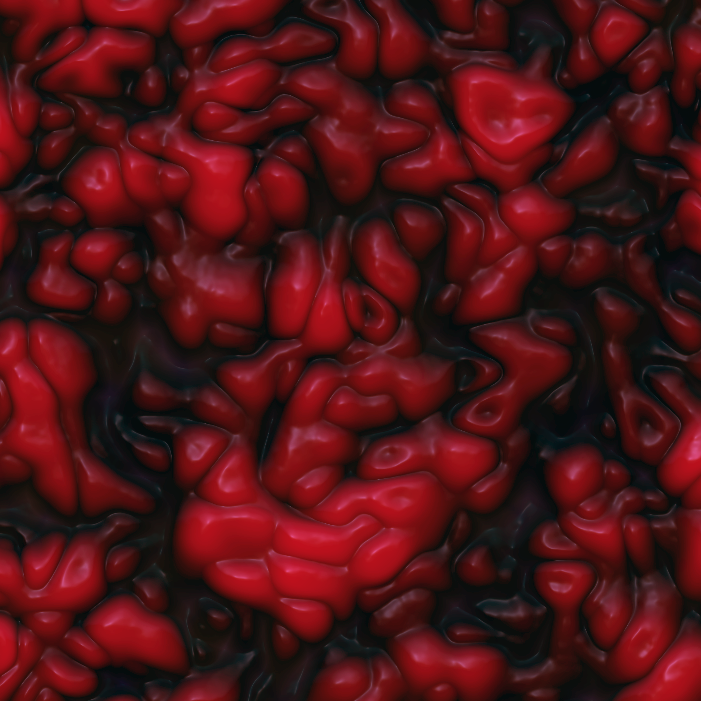
\includegraphics[scale=0.164]{img/redPerlin.png}
            \caption{Tejido orgánico.}
        \end{subfigure}
        \hfill
        \begin{subfigure}[b]{0.3\textwidth}
            \centering
            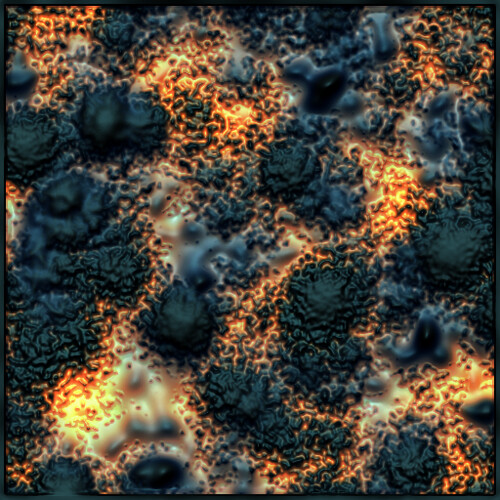
\includegraphics[scale=0.2305]{img/lavaPerlin.jpg}
            \caption{Terreno volcánico.}
        \end{subfigure}
        \hfill
        \begin{subfigure}[b]{0.3\textwidth}
            \centering
            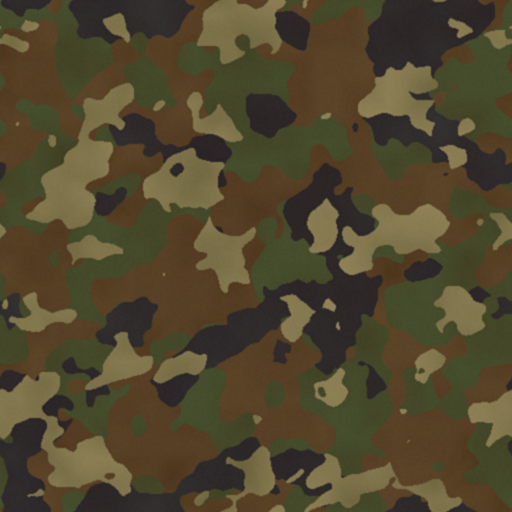
\includegraphics[scale=0.224]{img/camufaje.png}
            \caption{Patrón de camuflaje.}
        \end{subfigure}
        \caption{Texturas generadas utilizando ruido Perlin. Imágenes obtenidas de \cite{redPerlin}, \cite{lavaPerlin} y \cite{camuflajePerlin}.}
    \end{center}
\end{figure}

\paragraph{Métodos basados en búsqueda}
Estos métodos se basan en la generación de contenido seguida de una evaluación del mismo, puntuando su calidad. En estos métodos podemos identificar tres componentes: la representación del espacio, la función de evaluación y el algoritmo de búsqueda.

\begin{itemize}
    \item \textbf{Representación del espacio:} dependiendo del contenido generado y de la forma de generar dicho contenido, este contará con una representación. Las formas de representar estos datos pasan por vectores, matrices, árboles e incluso por un diseño específico para nuestro problema.
    \item \textbf{Función de evaluación:} será la encargada de evaluar la calidad de las soluciones obtenidas. Esta evaluación puede ser desde una función simple de combinaciones lineales de características (por ejemplo, en un laberinto, cuantos cruces tiene, si tiene caminos cerrados, etc.) o funciones complejas que utilicen modelos matemáticos para su optimización, como en el caso de las redes neuronales.
    \item \textbf{Algoritmo de búsqueda:} es el encargado de realizar una búsqueda en nuestra representación del espacio apoyándose en la función de evaluación para escoger los mejores individuos del espacio. Tal y como refleja Togelius \textit{et al.} \cite{togelius2011} el método más utilizado como algoritmo de búsqueda son los algoritmos evolutivos, aunque también se utilizan otros métodos como enfriamiento simulado, búsqueda local o cualquier otro tipo de metaheurística \cite{molina2020}.
\end{itemize}

Un gran ejemplo de aplicación de métodos basados en búsqueda para generar contenido es el experimento llevado a cabo por Togelius \textit{et al.} \cite{togelius2007} en el que generan de manera evolutiva circuitos para un juego de carreras.

\paragraph{Métodos de aprendizaje automático}

Recientemente diversos métodos de aprendizaje automático han demostrado ser capaces de generar contenido de juegos. Algunos ejemplos exitosos son la generación de nuevos niveles del videojuego Super Mario usando redes neuronales recursivas por Summerville \& Mateas \cite{summerville2016}, usando autoencoders por Jain \textit{et al.} \cite{jain2016} o usando modelos de Markov por Snodgrass \& Ontañón \cite{snodgrass2017}. Como se puede observar en el trabajo de Barriga \cite{barriga2019} y en los ejemplos recién expuestos, los métodos de aprendizaje automático se usan principalmente para la generación de niveles.

\begin{figure}[H]
    \begin{center}
        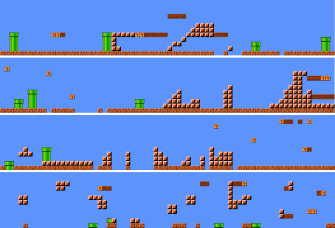
\includegraphics[scale=0.775]{img/mario.png}
        \caption{Niveles del videojuego Super Mario generados utilizando Modelos de Markov. Imagen obtenida de \cite{snodgrass2017}.}
    \end{center}
\end{figure}

% ---------------------------------------------------------------------------- %

\subsubsection{Recorrido histórico del uso de la PCG}

Los métodos de generación procedimental de contenido no solo se han usado en el ámbito de los videojuegos en la última década sino que su aplicación aparece ya a principio de la década de los 80. En este breve recorrido histórico seguiremos el primer capítulo del libro de Shaker \textit{et al.} \cite{shaker2016} y el trabajo de Amato \cite{amato2017}, sacando información sobre juegos que usan generación procedimental tanto de la web \textit{The Gamer} \cite{glenn2021} como de Wikipedia \cite{listWiki}. Además, podemos añadir una mención especial a \textit{Everything Procedural} \cite{EP}, la conferencia anual sobre generación procedimental aplicada a videojuegos.

\begin{table}[H]
    \centering
    \caption{Relación de videojuegos que usan PCG.}
    \begin{tabular}{|l|l|l|}
    \hline
    Videojuego & Lanzamiento & Contenido generado procedimentalmente \\ \hline
    Rogue      & 1980        & Niveles ASCII  \\ \hline
    Elite      & 1984        &     Planetas y galaxias   \\ \hline
    \textit{Saga} Civilation     & 1991-2018        & Niveles \acrshort{2d} y \acrshort{3d}   \\ \hline
    \textit{Saga} X-Com     & 1993-2016        &  Niveles \acrshort{2d} y \acrshort{3d}  \\ \hline
    Diablo     & 1996        & Niveles \acrshort{2d} y recompensas     \\ \hline
    KKrieger     & 2004        & Mallas, texturas y música     \\ \hline
    Dwarf Fortress & 2006 & Mapeado y ecosistemas \\ \hline
    The Elder Scrolls IV: Oblivion     & 2006        & Vegetación     \\ \hline
    Spelunky     & 2008        & Niveles \acrshort{2d}  \\ \hline
    Spore     & 2008        & Terreno, planetas, criaturas y animaciones \\ \hline
    \textit{Saga} Batman: Arkham     & 2009-2015        & Vegetación   \\ \hline
    \textit{Saga} Borderlands     & 2009-2019        & Armas   \\ \hline
    Left 4 Dead 2     & 2009        & Dificultad adaptativa   \\ \hline
    Minecraft     & 2011        & Mundo \acrshort{3d}      \\ \hline
    Elite: Dangerous     & 2015        & Planetas y galaxia \\ \hline
    Rogue Legacy &	2011 & Niveles \acrshort{2d} \\ \hline
    Terraria &	2011 & Mundo \acrshort{2d} \\ \hline
    \textit{Saga} The Binding of Isaac &	2011-2021 & Niveles \acrshort{2d}  \\ \hline
    Don't Starve &	2013 & Mundo \acrshort{2d} \\ \hline
    Crypt of the NecroDancer &	2015 & Niveles \acrshort{2d} \\ \hline
    Mini Metro &	2015 & Localización objetivos y recursos, y audio \\ \hline
    Darkest Dungeon & 2016 & Niveles \acrshort{2d} \\ \hline
    Enter the Gungeon & 2016 & Niveles \acrshort{2d} \\ \hline
    No Man's Sky & 2016 & Planetas, recursos, ecosistemas, criaturas, etc.  \\ \hline
    Bad North & 2018 & Niveles \acrshort{3d}  \\ \hline
    Into The Breach & 2018 & Niveles \acrshort{2d}\\ \hline
    Mini Motorways & 2019 & Localización objetivos y recursos \acrshort{3d} \\ \hline
    Townscaper & 2020 & Niveles \acrshort{3d} \\ \hline
    Valheim & 2021 & Mundo \acrshort{3d} \\ \hline
    \end{tabular}
\end{table}

\newpage

En 1980 se publicó \textit{Rogue} \cite{wichman1997}, uno de los primeros \textit{dungeon-crawlers} y el considerado ancestro de los juegos \textit{Rogue-like}\footnote{La traducción literal es "que se parece a Rogue", de ahí el nombre de esta categoría.} Esta categoría de juegos siempre utiliza algún tipo de generación procedimental ya que, tal y como ya pasaba en \textit{Rogue}, los niveles se generan aleatoriamente cada vez que comienza el juego.\\

\begin{figure}[H]
    \begin{center}
        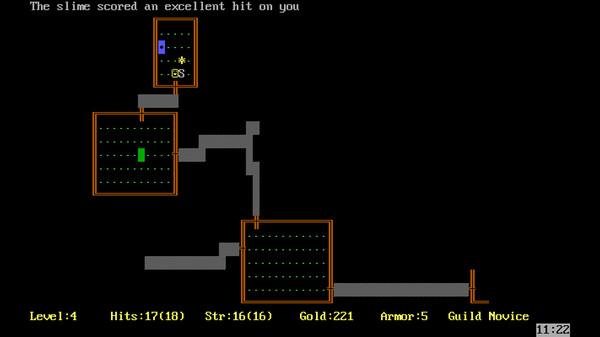
\includegraphics[scale=0.37]{img/rogue.jpg}
        \caption{Mazmorra generada procedimentalmente del videojuego \textit{Rogue}. Imagen obtenida de \cite{epyx}.}
    \end{center}
\end{figure}

Unos años más tarde, en 1984, se publicó \textit{Elite} \cite{braben2007} que estableció una solución para las capacidades limitadas de los ordenadores de 8 bits, generando procedimentalmente 256 planetas distribuidos en 8 galaxias mediante una semilla. Más tarde, en 2014 se publicó \textit{Elite: Dangerous}, una versión moderna del juego que usando \acrshort{pcg} te permite explorar una galaxia compuesta por 400 mil millones de sistemas estelares, números solo alcanzables gracias a la generación procedimental, como bien señala Amato \cite{amato2017}, ya que suponiendo que un sistema solar ocupase solamente 1\acrshort{KB}, el sistema representando en el juego ocuparía 40\acrshort{TB}.\\

\begin{figure}[H]
    \begin{center}
        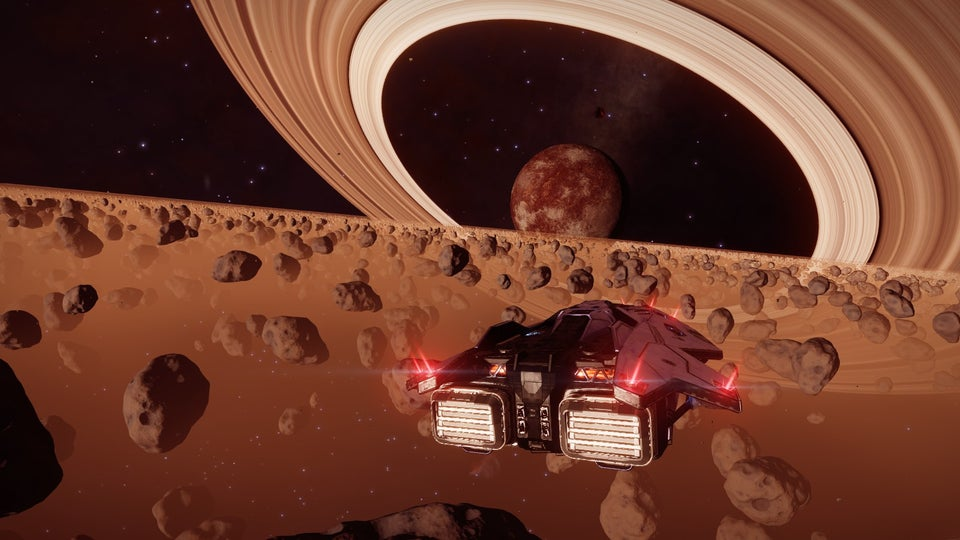
\includegraphics[scale=0.23]{img/elitedangerous.jpg}
        \caption{Planeta y cinturón de asteroides del videojuego \textit{Elite: Dangerous}. Imagen obtenida de \cite{eliteDangerous}.}
    \end{center}
\end{figure}

Más tarde, cuando comenzaron a desaparecer las limitaciones de espacio, aparecieron juegos como Diablo \cite{diablo}, un \textit{Rogue-like} híbrido que no solo generaba sus niveles procedimentalmente sino que implementó un sistema de recompensas que se generaban en el momento, sistema que se ha visto posteriormente en otros títulos como la saga de \textit{Borderlands}.\\

Poco a poco comenzó a usarse técnicas de \acrshort{pcg} con el fin de generar contenido más allá del nivelado del juego. Por ejemplo, el videojuego \textit{KKrieger} \cite{kosh} es un juego en \acrshort{3d} en primera persona publicado en 2004 que ocupa menos de 100\acrshort{KB} debido a que utiliza generación procedimental para crear las mallas de los modelos, las texturas e incluso la música.

\begin{figure}[H]
    \begin{center}
        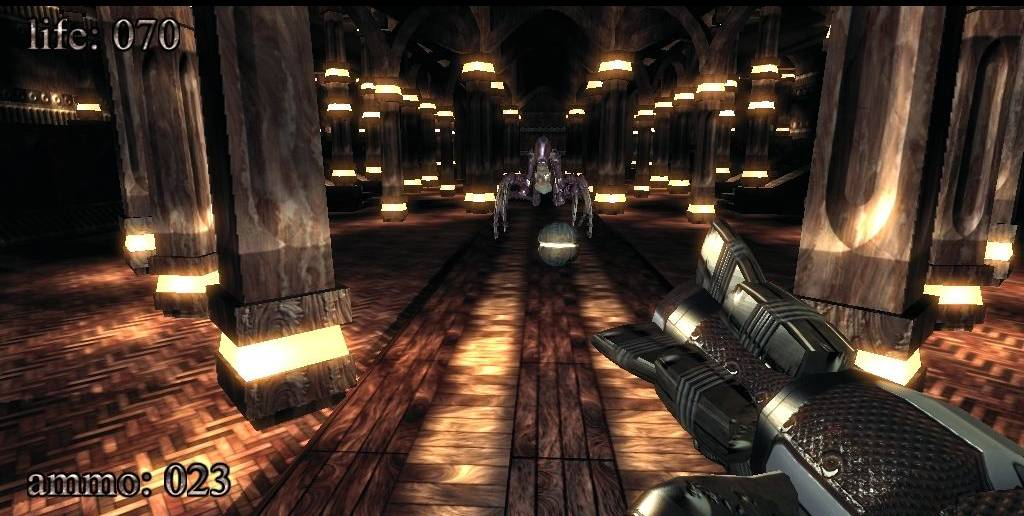
\includegraphics[scale=0.3]{img/kkrieger.jpg}
        \caption{Mazmorra generada procedimentalmente del videojuego \textit{Kkrieger}. Imagen obtenida de \cite{chirinea}.}
    \end{center}
\end{figure}

Aunque si hablamos de videojuegos que utilizan técnicas de \acrshort{pcg} como base fundamental de su jugabilidad no podemos evitar hablar de \textit{Spore} \cite{spore}, juego lanzado en 2008 en el que se generaba planetas, criaturas, terreno y otros elementos como las animaciones de las criaturas que se generan al momento, y de \textit{No Man's Sky} \cite{nomansky}, juego lanzado en 2016 que nos permite visitar 18 trillones de planetas ya que genera prácticamente la totalidad de su contenido procedimentalmente.

\begin{figure}[H]
    \centering
        \begin{subfigure}[b]{0.49\textwidth}
            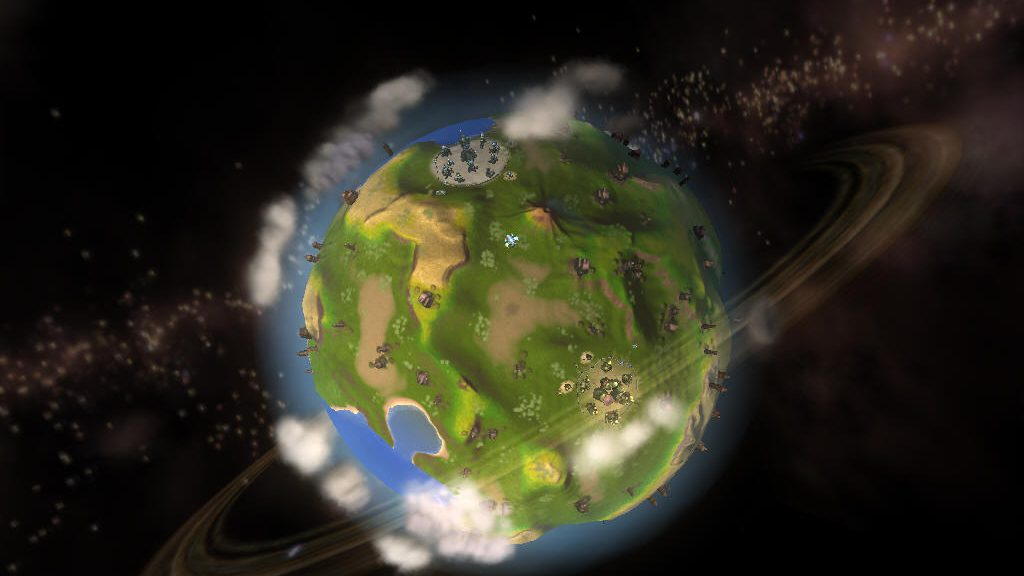
\includegraphics[width=\textwidth]{img/spore.jpg}
            \caption{Planeta del videojuego \textit{Spore}.}
        \end{subfigure}
        \hfill
        \begin{subfigure}[b]{0.49\textwidth}
            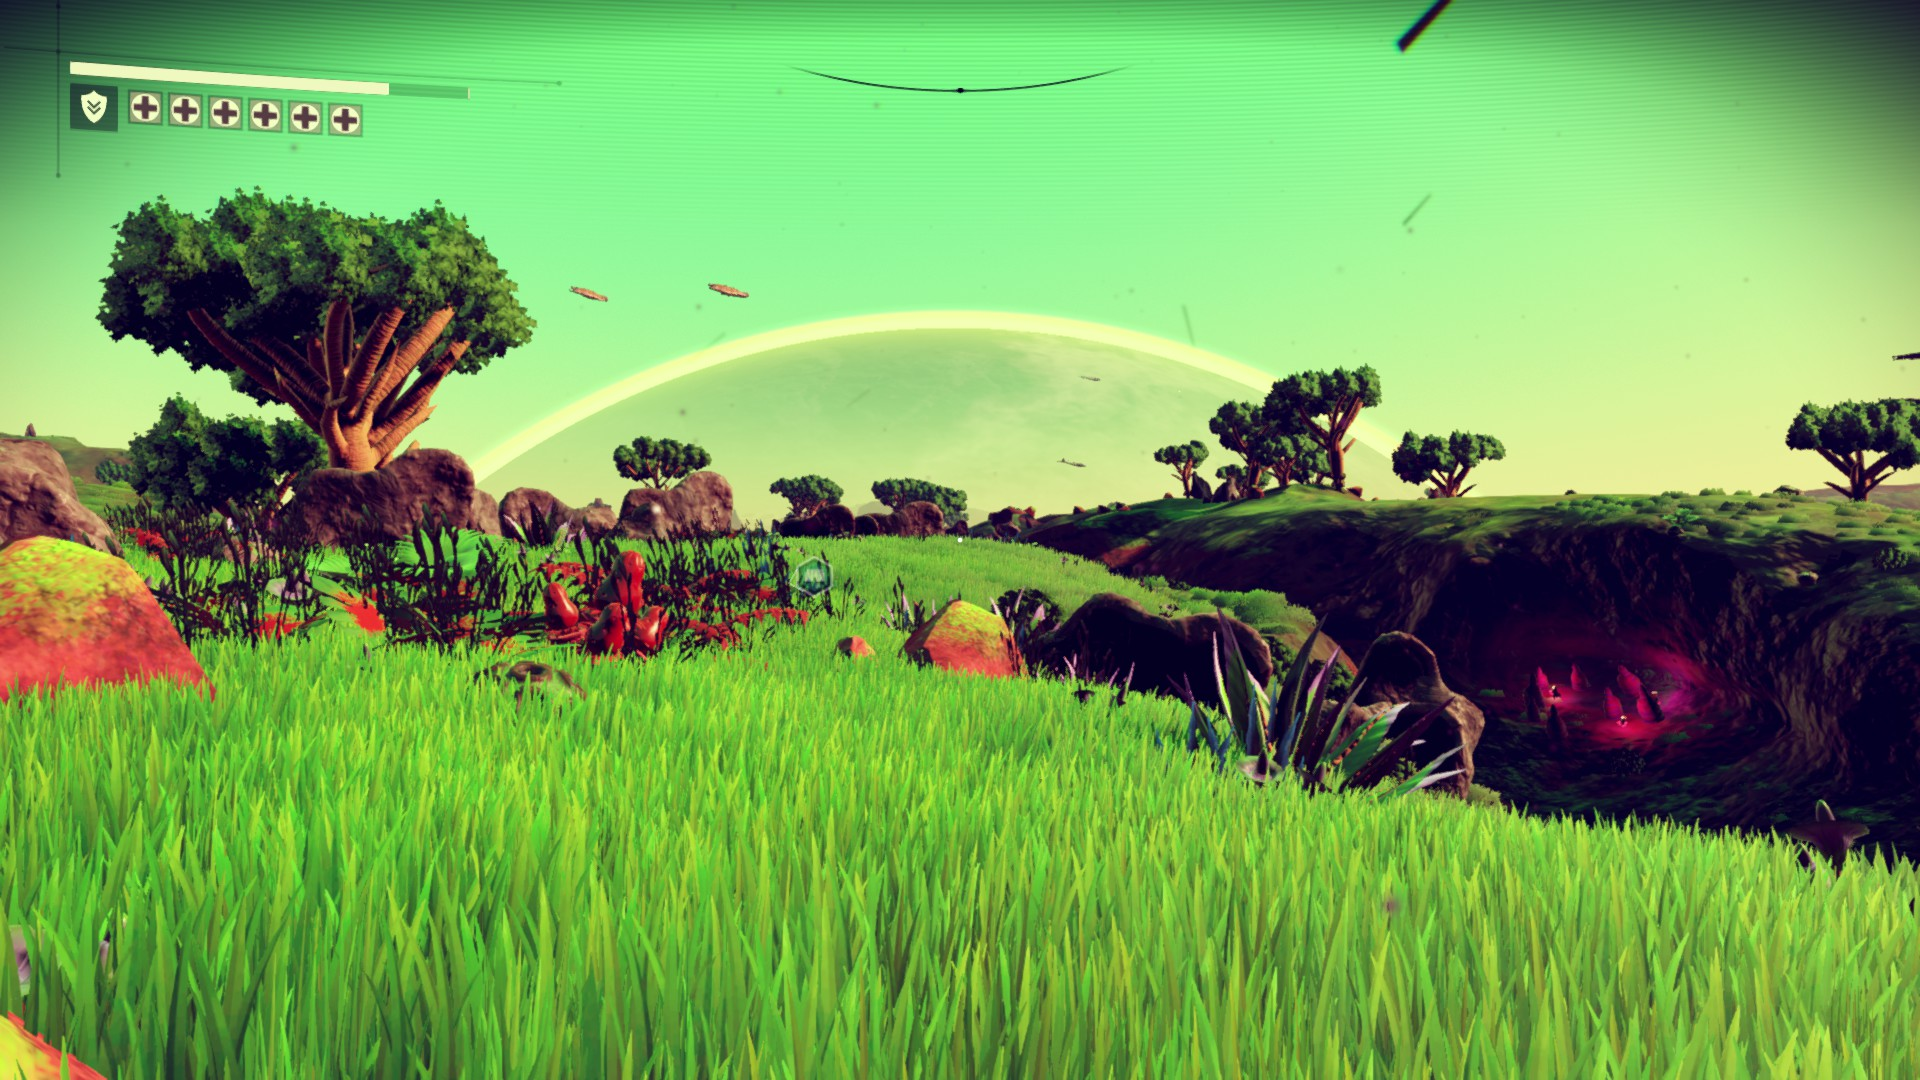
\includegraphics[width=\textwidth]{img/jake.jpeg}
            \caption{Planeta del videojuego \textit{No Man's Sky}.}
        \end{subfigure}
        \caption{Escenas de juegos que han basado elementos principales de su desarrollo en PCG. Imágenes obtenidas de \cite{spore} y \cite{jake}.}
\end{figure}

Con el tiempo se ha desarrollado incluso software específico para generar contenido especializado de manera procedimental, como ocurre con la herramienta \textit{SpeedTree} \cite{speedtree} que se ha especializado en generación y modelado de vegetación y se ha usado en juegos como la saga \textit{Batman: Arkham}, en \textit{The Elder Scrolls IV: Oblivion} o en el propio \textit{No Man's Sky}.\\

Sin embargo, aunque la generación procedimental se ha usado en diversos géneros y para generar multitud de contenido, se puede observar que dentro del mundo de los videojuegos el contenido más frecuentemente generado es el nivelado y mapeado, por ello los juegos \textit{Rogue-like} son los que mayoritariamente se benefician de y aplican técnicas de generación procedimental. Esto se puede observar en el catálogo de videojuegos que han utilizado \acrshort{pcg} como un elemento principal de su diseño.\\

Contamos con multitud de ejemplos de juegos que cumplen con esto, entre ellos, \textit{Rogue Legacy} o \textit{Darkest Dungeon}, que al más puro estilo de original \textit{Rogue} nos permite recorrer una \acrshort{2d} diferente cada vez que comencemos una nueva misión; otros como \textit{Crypt of the NecroDancer} o \textit{Into The Breach}, que combinan la rejugabilidad y variedad que aporta la generación procedimental con mecánicas ya conocidas pero novedosas en este nicho, siendo el primero un juego de ritmo y el segundo un juego de puzzles; e incluso juegos que su atractivo principal es el uso de generación procedimental, tal y como hace \textit{Townscaper} cuya jugabilidad se basa en diseñar ciudades generadas procedimentalmente.\\

\begin{figure}[H]
    \begin{center}
        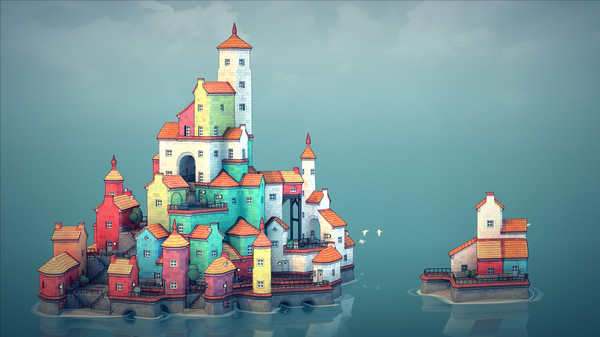
\includegraphics[scale=0.4]{img/town.jpg}
        \caption{Ciudad generada procedimentalmente por un jugador en el juego \textit{Townscaper}. Imagen obtenida de \cite{oscar}.}
    \end{center}
\end{figure}